\chapter{Data collection}
\label{introductionToData}

%\begin{tipBox}{\tipBoxTitle[Chapter Goal:]{Thinking about data}
%Understand basics about data organization, data types, numerical summaries of data, graphical summaries of data, and foundational techniques for data collection. We begin and end the chapter with case studies.}
%\end{tipBox}

Scientists seek to answer questions using rigorous methods and careful observations. These observations -- collected from the likes of field notes, surveys, and experiments -- form the backbone of a statistical investigation and are called \term{data}. Statistics is the study of how best to collect, analyze, and draw conclusions from data. It is helpful to put statistics in the context of a general process of investigation:
\begin{enumerate}
\setlength{\itemsep}{0mm}
\item Identify a question or problem.
\item Collect relevant data on the topic.
\item Analyze the data.
\item Form a conclusion.
%\item Make decisions based on the conclusion.
\end{enumerate}

Statistics as a subject focuses on making stages 2-4 objective, rigorous, and efficient. That~is, statistics has three primary components: How best can we collect data? How should it be analyzed? And what can we infer from the analysis?

\Add{
Researchers from a wide array of fields have questions or problems that require the collection and analysis of data. Let's consider three examples. 
\begin{itemize}
\item Climate scientists: how will the global temperature change over the next 100 years?
\item Psychology: can a simple reminder about saving money cause students to spend less?
\item Political science: what fraction of Americans approve of the job Congress is doing?
\end{itemize}
}
While the questions that can be posed are incredibly diverse, many of these investigations can be addressed with a small number of data collection techniques, analytic tools, and fundamental concepts in statistical inference. \Comment{this is my next attempt at writing something that tries to excite the students about the book, especially this first chapter}\Add{This chapter focuses on stage 2, collecting data.  We'll discuss basic properties of data, common sources of bias that arise during data collection, and several techniques for collecting data through both sampling techniques and experiments. After finishing this chapter, you will have the tools for identifying weaknesses and strengths in data-based conclusions, tools that are essential to be an informed citizen and a savvy consumer of information.} \Cut{For example, you may begin to identify exaggerated claims made by journalists or bloggers}

\Cut{Do not be surprised if, upon finishing this chapter, you find yourself questioning and approaching everything you read with a critical eye.  Indeed, the practice of statistics invites and demands us to do just that.}   \Cut{This chapter provides a glimpse into these and other themes we will encounter throughout the rest of the book. We introduce the basic principles of each branch and learn some tools along the way. We will encounter applications from other fields, some of which are not typically associated with science but nonetheless can benefit from statistical study.}


\section[Case study]{Case study: using stents to prevent strokes}
\label{basicExampleOfStentsAndStrokes}

\index{data!stroke|(}

Section~\ref{basicExampleOfStentsAndStrokes} introduces a classic challenge in statistics: evaluating the efficacy of a medical treatment. Terms in this section, and indeed much of this chapter, will all be revisited later in the text. The plan for now is simply to get a sense of the role statistics can play in practice.

In this section we will consider an experiment that studies effectiveness of stents in treating patients at risk of stroke.\footnote{Chimowitz MI, Lynn MJ, Derdeyn CP, et al. 2011. Stenting versus Aggressive Medical Therapy for Intracranial Arterial Stenosis. New England Journal of Medicine 365:993-1003. \urlwofont{http://www.nejm.org/doi/full/10.1056/NEJMoa1105335}. NY Times article reporting on the study: \urlwofont{http://www.nytimes.com/2011/09/08/health/research/08stent.html}.} Stents are devices put inside blood vessels that assist in patient recovery after cardiac events and reduce the risk of an additional heart attack or death. Many doctors have hoped that there would be similar benefits for patients at risk of stroke. We start by writing the principal question the researchers hope to answer:
\begin{quote}
Does the use of stents reduce the risk of stroke?
\end{quote}

The researchers who asked this question collected data on 451 at-risk patients. Each volunteer patient was randomly assigned to one of two groups:
\begin{itemize}
\item[]\termsub{Treatment group}{treatment group}. Patients in the treatment group received a stent and medical management. The medical management included medications, management of risk factors, and help in lifestyle modification. 
\item[]\termsub{Control group}{control group}. Patients in the control group received the same medical management as the treatment group, but they did not receive stents.
\end{itemize}
Researchers randomly assigned 224 patients to the treatment group and 227 to the control group. In this study, the control group provides a reference point against which we can measure the medical impact of stents in the treatment group.

Researchers studied the effect of stents at two time points: 30~days after enrollment and 365~days after enrollment. The results of 5 patients are summarized in Table~\ref{stentStudyResultsDF}. Patient outcomes are recorded as ``stroke'' or ``no event'', representing whether or not the patient had a stroke at the end of a time period.

\begin{table}[h]
\centering
\begin{tabular}{l ccc}
\hline
Patient	&	group	&	0-30 days 	&	0-365 days \\
\hline
1		&	treatment &	no event &	no event \\
2		&	treatment &	stroke & stroke \\
3		&	treatment &	no event & no event \\
$\vdots$	&	$\vdots$	  &	$\vdots$ \\
450	&	control &	no event &	no event \\
451	&	control &	no event &	no event \\
\hline
\end{tabular}
\caption{Results for five patients from the stent study.}
\label{stentStudyResultsDF}
% trmt <- c(rep('trmt', 224), rep('control', 227)); outcome30 <- c(rep(c('event', 'no_event'), c(33, 191)), rep(c('event', 'no_event'), c(13, 214))); outcome365 <- c(rep(c('event', 'no_event'), c(33, 191)), rep(c('event', 'no_event'), c(13, 214)))
\end{table}

Considering data from each patient individually would be a long, cumbersome path towards answering the original research question. Instead, performing a statistical data analysis allows us to consider all of the data at once. Table~\ref{stentStudyResults} summarizes the raw data in a more helpful way. In this table, we can quickly see what happened over the entire study. For instance, to identify the number of patients in the treatment group who had a stroke within 30 days, we look on the left-side of the table at the intersection of the treatment and stroke: 33.

\begin{table}[h]
\centering
\begin{tabular}{l cc c cc}
& \multicolumn{2}{c}{0-30 days} &\hspace{5mm}\ & \multicolumn{2}{c}{0-365 days} \\
  \cline{2-3} \cline{5-6}
	& 	stroke 	& no event && 	stroke 	& no event \\
  \hline
treatment 	& 33		& 191	&&	45 	& 179 \\
control 		& 13		& 214	&& 	28	& 199 \\
  \hline
Total				& 46		& 405	&&	73	& 378 \\
  \hline
\end{tabular}
\caption{Descriptive statistics for the stent study.}
\label{stentStudyResults}
\end{table}

\begin{exercise}
Of the 224 patients in the treatment group, 45 had a stroke by the end of the first year. Using these two numbers, compute the proportion of patients in the treatment group who had a stroke by the end of their first year. (Please note: answers to all in-text exercises are provided using footnotes.)\footnote{The proportion of the 224 patients who had a stroke within 365 days: $45/224 = 0.20$.}
\end{exercise}

We can compute summary statistics from the table. A \term{summary statistic} is a single number summarizing a large amount of data.\footnote{Formally, a summary statistic is a value computed from the data. Some summary statistics are more useful than others.} For instance, the primary results of the study after 1~year could be described by two summary statistics: the proportion of people who had a stroke in the treatment and control groups.
\begin{itemize}
\setlength{\itemsep}{0mm}
\item[] Proportion who had a stroke in the treatment (stent) group: $45/224 = 0.20 = 20\%$.
\item[] Proportion who had a stroke in the control group: $28/227 = 0.12 = 12\%$.
\end{itemize}
These two summary statistics are useful in looking for differences in the groups, and we are in for a surprise: an additional 8\% of patients in the treatment group had a stroke! This is important for two reasons. First, it is contrary to what doctors expected, which was that stents would \emph{reduce} the rate of strokes. Second, it leads to a statistical question: do the data show a ``real'' difference between the groups?

This second question is subtle. Suppose you flip a coin 100 times. While the chance a coin lands heads in any given coin flip is 50\%, we probably won't observe exactly 50 heads. This type of fluctuation is part of almost any type of data generating process. It is possible that the 8\% difference in the stent study is due to this natural variation. However, the larger the difference we observe (for a particular sample size), the less believable it is that the difference is due to chance. So what we are really asking is the following: is the difference so large that we should reject the notion that it was due to chance?

While we don't yet have our statistical tools to fully address this question on our own, we can comprehend the conclusions of the published analysis: there was compelling evidence of harm by stents in this study of stroke patients.

\textbf{Be careful:} do not generalize the results of this study to all patients and all stents. This study looked at patients with very specific characteristics who volunteered to be a part of this study and who may not be representative of all stroke patients. In addition, there are many types of stents and this study only considered the self-expanding Wingspan stent (Boston Scientific). However, this study does leave us with an important lesson: we should keep our eyes open for surprises.

\index{data!stroke|)}

\section{Data basics}
\label{dataBasics}

Effective presentation and description of data is a first step in most analyses. This section introduces one structure for organizing data as well as some terminology that will be used throughout this book.

\subsection{Observations, variables, and data matrices}

\index{data!email50|(}

Table~\ref{email50DF} displays rows 1, 2, 3, and 50 of a data set concerning 50 emails received during early 2012. These observations will be referred to as the \data{email50} data set, and they are a random sample from a larger data set that we will see in Section~\ref{categoricalData}.

Each row in the table represents a single email or \term{case}.\footnote{A case is also sometimes called a \term{unit of observation} or an \term{observational unit}.} The columns represent characteristics, called \termsub{variables}{variable}, for each of the emails. For example, the first row represents email 1, which is a not spam, contains 21,705 characters, 551 line breaks, is written in HTML format, and contains only small numbers.

In practice, it is especially important to ask clarifying questions to ensure important aspects of the data are understood. For instance, it is always important to be sure we know what each variable means and the units of measurement. Descriptions of all five email variables are given in Table~\ref{email50Variables}.

\begin{table}[t]
\centering
\begin{tabular}{cc ccc c}
  \hline
 & \var{spam} & \var{num\_\hspace{0.3mm}char} & \var{line\_\hspace{0.3mm}breaks} & \var{format} & \var{number} \\ 
  \hline
1 & no & 21,705 & 551 & html & small \\ 
  2 & no & 7,011 & 183 & html & big \\ 
  3 & yes & 631 & 28 & text & none \\ 
$\vdots$ & $\vdots$ & $\vdots$ & $\vdots$ & $\vdots$ & $\vdots$ \\
  50 & no & 15,829 & 242 & html & small \\ 
   \hline
\end{tabular}
\caption{Four rows from the \data{email50} data matrix.}
\label{email50DF}
\end{table}
% library(openintro); library(xtable); data(email50); email50[c(1,2,3,50),c("spam", "num_char", "line_breaks", "format", "number")]; xtable(email50[c(1,2,3,50),c("spam", "num_char", "line_breaks", "format", "number")], digits=0)


\begin{table}[t]
\centering\small
\begin{tabular}{lp{10.5cm}}
\hline
{\bf variable} & {\bf description} \\
\hline
\var{spam} & Specifies whether the message was spam \\
\var{num\_\hspace{0.3mm}char} & The number of characters in the email   \\
\var{line\_\hspace{0.3mm}breaks} & The number of line breaks in the email (not including text wrapping)   \\
\var{format} & Indicates if the email contained special formatting, such as bolding, tables, or links, which would indicate the message is in HTML format    \\
\var{number} & Indicates whether the email contained no number, a small number (under 1 million), or a large number   \\
\hline
\end{tabular}
\caption{Variables and their descriptions for the \data{email50} data set.\vspaceB{-3.5mm}}
\label{email50Variables}
\end{table}

\index{data!email50|)}

The data in Table~\ref{email50DF} represent a \term{data matrix}, which is a common way to organize data. Each row of a data matrix corresponds to a unique case, and each column corresponds to a variable. A data matrix for the stroke study introduced in Section~\ref{basicExampleOfStentsAndStrokes} is shown in Table~\vref{stentStudyResultsDF}, where the cases were patients and there were three variables recorded for each patient.

Data matrices are a convenient way to record and store data. If another individual or case is added to the data set, an additional row can be easily added. Similarly, another column can be added for a new variable.

\index{data!county|(}

\begin{exercise}
We consider a publicly available data set that summarizes information about the 3,143 counties in the United States, and we call this the \data{county} data set. This data set includes information about each county: its name, the state where it resides, its population in 2000 and 2010, per capita federal spending, poverty rate, and five additional characteristics. How might these data be organized in a data matrix? Reminder: look in the footnotes for answers to in-text exercises.\footnote{Each county may be viewed as a case, and there are eleven pieces of information recorded for each case. A table with 3,143 rows and 11 columns could hold these data, where each row represents a county and each column represents a particular piece of information.}
\end{exercise}

\noindent Seven rows of the \data{county} data set are shown in Table~\ref{countyDF}, and the variables are summarized in Table~\ref{countyVariables}. These data were collected from the US Census website.\footnote{\urlwofont{http://quickfacts.census.gov/qfd/index.html}}

\begin{landscape}
\begin{table}
\centering\small
\begin{tabular}{ccc ccc ccc ccc}
\hline
& \var{name} & \var{state} & \var{pop2000} & \var{pop2010} &
   \var{fed\_\hspace{0.3mm}spend} & \var{poverty} & \var{homeownership} & \var{multiunit} &
   \var{income} & \var{med\_\hspace{0.3mm}income} & \var{smoking\_\hspace{0.3mm}ban} \\
\hline
  1 & Autauga & AL & 43671 & 54571 & 6.068 & 10.6 & 77.5 & 7.2 & 24568 & 53255 & none \\
  2 & Baldwin & AL & 140415 & 182265 & 6.140 & 12.2 & 76.7 & 22.6 & 26469 & 50147 & none \\ 
  3 & Barbour & AL & 29038 & 27457 & 8.752 & 25.0 & 68.0 & 11.1 & 15875 & 33219 & none \\ 
  4 & Bibb & AL & 20826 & 22915 & 7.122 & 12.6 & 82.9 & 6.6 & 19918 & 41770 & none \\ 
  5 & Blount & AL & 51024 & 57322 & 5.131 & 13.4 & 82.0 & 3.7 & 21070 & 45549 & none \\ 
  $\vdots$ & $\vdots$ & $\vdots$ & $\vdots$ & $\vdots$ & $\vdots$ & $\vdots$ & $\vdots$ & $\vdots$ & $\vdots$ & $\vdots$ & $\vdots$ \\
  3142 & Washakie & WY & 8289 & 8533 & 8.714 & 5.6 & 70.9 & 10.0 & 28557 & 48379 & none \\ 
  3143 & Weston & WY & 6644 & 7208 & 6.695 & 7.9 & 77.9 & 6.5 & 28463 & 53853 & none \\ 
\hline
\end{tabular}
\caption{Seven rows from the \data{county} data set.}
\label{countyDF}
% library(openintro); county <- countyComplete[,c("name", "state", "pop2000", "pop2010", "fed_spending", "poverty", "home_ownership", "housing_multi_unit", "per_capita_income", "median_household_income")]; colnames(county) <- c("name", "state", "pop2000", "pop2010", "fed_spend", "poverty", "homeownership", "multiunit", "income", "med_income"); county$fed_spend <- county$fed_spend / county$pop2010

% library(openintro); library(xtable); cc <- countyComplete; xtable(cc[c(1:5,nrow(cc) - (1:0)), c("name", "state", "pop2000", "pop2010", "fed_spend", "poverty", "homeownership", "multiunit", "income", "med_income")], digits=1)
\end{table}

\begin{table}
\centering\small
\begin{tabular}{lp{11cm}}
\hline
{\bf variable} & {\bf description} \\
\hline
\var{name} & County name \\
\var{state} & State where the county resides (also including the District of Columbia) \\
\var{pop2000} & Population in 2000 \\
\var{pop2010} & Population in 2010 \\
\var{fed\_\hspace{0.3mm}spend} & Federal spending per capita \\
\var{poverty}  &  Percent of the population in poverty \\
\var{homeownership}  &  Percent of the population that lives in their own home or lives with the owner (e.g. children living with parents who own the home) \\
\var{multiunit}  &  Percent of living units that are in multi-unit structures (e.g. apartments) \\
\var{income} & Income per capita \\
\var{med\_\hspace{0.3mm}income} & Median household income for the county, where a household's income equals the total income of its occupants who are 15 years or older \\
\var{smoking\_\hspace{0.3mm}ban}  &  Type of county-wide smoking ban in place at the end of 2011, which takes
			one of three values: \resp{none}, \resp{partial}, or \resp{comprehensive},
			where a \resp{comprehensive} ban means smoking
			was not permitted in restaurants, bars, or workplaces, and \resp{partial}
			means smoking was banned in at least one of those three locations \\
\hline
\end{tabular}
\centering
\caption{Variables and their descriptions for the \data{county} data set.}
\label{countyVariables}
\end{table}
\end{landscape}

\subsection{Types of variables}
\label{variableTypes}

Examine the \var{fed\_\hspace{0.3mm}spend}, \var{pop2010}, \var{state}, and \var{smoking\_\hspace{0.3mm}ban} variables in the \data{county} data set. Each of these variables is inherently different from the other three yet many of them share certain characteristics.

First consider \var{fed\_\hspace{0.3mm}spend}, which is said to be a \term{numerical} variable since it can take a wide range of numerical values, and it is sensible to add, subtract, or take averages with those values. On the other hand, we would not classify a variable reporting telephone area codes as numerical since their average, sum, and difference have no clear meaning.

The \var{pop2010} variable is also numerical, although it seems to be a little different than \var{fed\_\hspace{0.3mm}spend}. This variable of the population count can only take whole non-negative numbers (\resp{0}, \resp{1}, \resp{2}, ...). For this reason, the population variable is said to be \term{discrete} since it can only take numerical values with jumps. On the other hand, the federal spending variable is said to be \term{continuous}.

The variable \var{state} can take up to 51 values after accounting for Washington, DC: \resp{AL}, ..., and \resp{WY}. Because the responses themselves are categories, \var{state} is called a \term{categorical} variable,\footnote{Sometimes also called a \term{nominal} variable.} and the possible values are called the variable's \term{levels}.

\begin{figure}
\centering
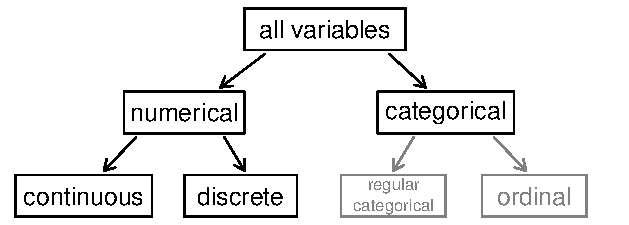
\includegraphics[width=0.57\textwidth]{01/figures/variables/variables}
\caption{Breakdown of variables into their respective types.}
\label{variables}
\end{figure}

Finally, consider the \var{smoking\_\hspace{0.3mm}ban} variable, which describes the type of county-wide smoking ban and takes values \resp{none}, \resp{partial}, or \resp{comprehensive} in each county. This variable seems to be a hybrid: it is a categorical variable but the levels have a natural ordering. A variable with these properties is called an \term{ordinal} variable. To simplify analyses, any ordinal variables in this book will be treated as categorical variables.

\begin{example}{Data were collected about students in a statistics course. Three variables were recorded for each student: number of siblings, student height, and whether the student had previously taken a statistics course. Classify each of the variables as continuous numerical, discrete numerical, or categorical.}
The number of siblings and student height represent numerical variables. Because the number of siblings is a count, it is discrete. Height varies continuously, so it is a continuous numerical variable. The last variable classifies students into two categories -- those who have and those who have not taken a statistics course -- which makes this variable categorical.
\end{example}

\begin{exercise} \index{data!stroke}
Consider the variables \var{group} and \var{outcome} (at 30 days) from the stent study in Section~\ref{basicExampleOfStentsAndStrokes}. Are these numerical or categorical variables?\footnote{There are only two possible values for each variable, and in both cases they describe categories. Thus, each are categorical variables.}
\end{exercise}

\subsection{Relationships between variables}
\label{variableRelations}

Many analyses are motivated by a researcher looking for a relationship between two or more variables. A social scientist may like to answer some of the following questions:
\begin{enumerate}
\setlength{\itemsep}{0mm}
\item[(1)]\label{fedSpendingPovertyQuestion} Is federal spending, on average, higher or lower in counties with high rates of poverty?
\item[(2)]\label{ownershipMultiUnitQuestion} If homeownership is lower than the national average in one county, will the percent of multi-unit structures in that county likely be above or below the national average?
\item[(3)]\label{isAverageIncomeAssociatedWithSmokingBans} Which counties have a higher average income: those that enact one or more smoking bans or those that do not?
\end{enumerate}

To answer these questions, data must be collected, such as the \data{county} data set shown in Table~\ref{countyDF}. Examining summary statistics \index{summary statistic} could provide insights for each of the three questions about counties. Additionally, graphs can be used to visually summarize data and are useful for answering such questions as well.

\indexthis{Scatterplots}{scatterplot} are one type of graph used to study the relationship between two numerical variables. Figure~\ref{county_fed_spendVsPoverty} compares the variables \var{fed\_\hspace{0.3mm}spend} and \var{poverty}. Each point on the plot represents a single county. For instance, the highlighted dot corresponds to County~1088 in the \data{county} data set: Owsley County, Kentucky, which had a poverty rate of 41.5\% and federal spending of \$21.50 per capita. The scatterplot suggests a relationship between the two variables: counties with a high poverty rate also tend to have slightly more federal spending. We might brainstorm as to why this relationship exists and investigate each idea to determine which is the most reasonable explanation.

\begin{figure}
\centering
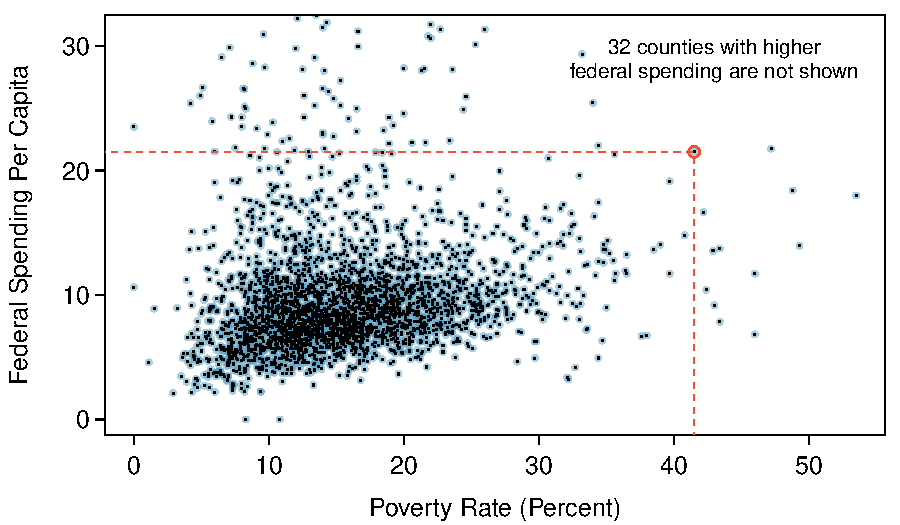
\includegraphics[width=0.8\textwidth]{01/figures/county_fed_spendVsPoverty/county_fed_spendVsPoverty}
\caption{A scatterplot showing \var{fed\_\hspace{0.3mm}spend} against \var{poverty}. Owsley County of Kentucky, with a poverty rate of 41.5\% and federal spending of \$21.50 per capita, is highlighted.}
\label{county_fed_spendVsPoverty}
\end{figure}

\begin{exercise}
Examine the variables in the \data{email50} data set, which are described in Table~\vref{email50Variables}. Create two questions about the relationships between these variables that are of interest to you.\footnote{Two sample questions: (1) Intuition suggests that if there are many line breaks in an email then there would tend to also be many characters: does this hold true? (2)~Is there a connection between whether an email format is plain text (versus HTML) and whether it is a spam message?}
\end{exercise}

The \var{fed\_\hspace{0.3mm}spend} and \var{poverty} variables are said to be associated because the plot shows a discernible pattern. When two variables show some connection with one another, they are called \term{associated} variables. Associated variables can also be called \term{dependent} variables and vice-versa.

\begin{example}{This example examines the relationship between homeownership and the percent of units in multi-unit structures (e.g. apartments, condos), which is visualized using a scatterplot in Figure~\ref{multiunitsVsOwnership}. Are these variables associated?}
It appears that the larger the fraction of units in multi-unit structures, the lower the homeownership rate. Since there is some relationship between the variables, they are associated.
\end{example}


\begin{figure}
   \centering
   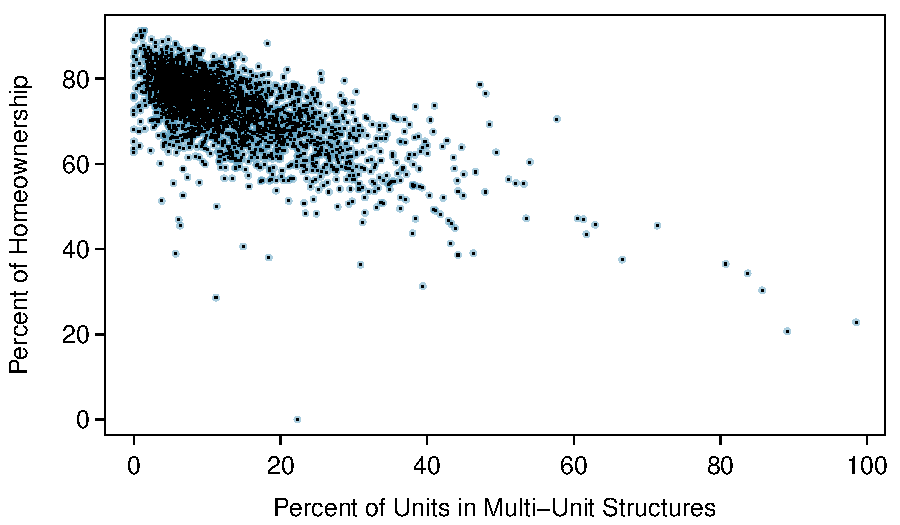
\includegraphics[width=0.8\textwidth]{01/figures/multiunitsVsOwnership/multiunitsVsOwnership}
   \caption{A scatterplot of homeownership versus the percent of units that are in multi-unit structures for all 3,143 counties. Interested readers may find an image of this plot with an additional third variable, county population, presented at \href{http://www.openintro.org/stat/down/MHP.png}{www.openintro.org/stat/down/MHP.png}.}
   \label{multiunitsVsOwnership}
\end{figure}

Because there is a downward trend in Figure~\ref{multiunitsVsOwnership} -- counties with more units in multi-unit structures are associated with lower homeownership -- these variables are said to be \termsub{negatively associated}{negative association}. A \term{positive association} is shown in the relationship between the \var{poverty} and \var{fed\_\hspace{0.3mm}spend} variables represented in Figure~\ref{county_fed_spendVsPoverty}, where counties with higher poverty rates tend to receive more federal spending per capita.

If two variables are not associated, then they are said to be \term{independent}. That is, two variables are independent if there is no evident relationship between the two.

\begin{termBox}{\tBoxTitle{Associated or independent, not both}
A pair of variables are either related in some way (associated) or not (independent). No pair of variables is both associated and independent.}
\end{termBox}

\index{data!county|)}

%%%%%
\section{Overview of data collection principles}
\label{overviewOfDataCollectionPrinciples}

\index{sample|(}
\index{population|(}
\index{parameter|(}
\index{statistic|(}

The first step in conducting research is to identify topics or questions that are to be investigated. A clearly laid out research question is helpful in identifying what subjects or cases should be studied and what variables are important. It is also important to consider \emph{how} data are collected so that they are reliable and help achieve the research goals.

\subsection{Populations and samples}
\label{populationsAndSamples}

Consider the following three research questions:
\begin{enumerate}
\setlength{\itemsep}{0mm}
\item What is the average mercury content in swordfish in the Atlantic Ocean?
\item\label{timeToGraduationQuestionForUCLAStudents} Over the last 5 years, what is the average time to complete a degree for Duke undergraduate students?
\item\label{identifyPopulationOfStentStudy} Does a new drug reduce the number of deaths in patients with severe heart disease?
\end{enumerate}
Each research question refers to a target \term{population}. In the first question, the target population is all swordfish in the Atlantic ocean, and each fish represents a case. Often times, it is too expensive to collect data for every case in a population. Instead, a sample is taken. A \term{sample} represents a subset of the cases and is often a small fraction of the population. For instance, 60 swordfish (or some other number) in the population might be selected, and this sample data may be used to provide an estimate of the population average and answer the research question.

\begin{exercise} \label{identifyingThePopulationForTwoQuestionsInPopAndSampSubsection}
For the second and third questions above, identify the target population and what represents an individual case.\footnote{(\ref{timeToGraduationQuestionForUCLAStudents}) Notice that the first question is only relevant to students who complete their degree; the average cannot be computed using a student who never finished her degree. Thus, only Duke undergraduate students who have graduated in the last five years represent cases in the population under consideration. Each such student would represent an individual case. (\ref{identifyPopulationOfStentStudy}) A person with severe heart disease represents a case. The population includes all people with severe heart disease.}
\end{exercise}

\Add{
We collect a sample of data to better understand the characteristics of a population. A \term{variable} is a characteristic we measure for each individual or case.  The overall quantity of interest may be the mean, median, proportion, or some other summary of a population. These population values are called \termsub{parameters}{parameter}. We estimate the value of a parameter by taking a sample and computing a numerical summary called a \term{statistic} based on that sample.  Note that the two p's (population, parameter) go together and the two s's (sample, statistic) go together.    

\begin{example}{Earlier we asked the question: what is the average mercury content in swordfish in the Atlantic Ocean? Identify the variable to be measured and the parameter and statistic of interest.}The variable is the amount of mercury content in swordfish in the Atlantic Ocean.  It will be measured for each individual swordfish. The parameter of interest is the average mercury content in \emph{all} swordfish in the Atlantic Ocean.  If we take a sample of 50 swordfish from the Atlantic Ocean, the average mercury content among just those 50 swordfish will be the statistic.
\end{example}  

Two statistics we will study are the \term{mean} (also called the \term{average}) and \term{proportion}. When we are discussing a population, we label the mean as $\mu$ (the Greek letter, \emph{mu}), while we label the sample mean as $\bar{x}$. When we are discussing a proportion in the context of a population, we use the label $p$, while the sample proportion has a label of $\hat{p}$ (read as \emph{p-hat}). Generally, we use $\bar{x}$ to estimate the population mean, $\mu$. Likewise, we use the sample proportion $\hat{p}$ to estimate the population proportion, $p$.

\Comment{possibly a table or figure here? }
\begin{example}{Is $\mu$ a parameter or statistic?  What about $\hat{p}$?}$\mu$ is a parameter because it refers to the average of the \emph{entire} population.  $\hat{p}$ is a statistic because it is calculated from a sample.
\end{example}

\begin{example}{For the second question regarding time to degree for a Duke undergraduate, is the variable numerical or categorical?  What is the parameter of interest?}The variable is numerical.  The characteristic that we record on each individual is the number of years until graduation.  The parameter of interest is the average time to degree for a Duke undergraduate.  We would use $\mu$ to describe this quantity.
\end{example}  

\begin{exercise}The third question asked whether a new drug reduces deaths in patients with severe heart disease.  Is the variable numerical or categorical?  Describe the statistic that should be calculated in this study. \footnote{The variable is whether or not a patient with severe heart disease dies within the time frame of the study.  This is categorical because it will be a yes or a no.  The statistic that should be recorded is the proportion of patients that die within the time frame of the study.  We would use $\hat{p}$ to denote this quantity. }
\end{exercise}

If these topics are still a bit unclear, don't worry. We'll cover them in greater detail in the next Chapter.
}

\subsection{Anecdotal evidence}
\label{anecdotalEvidenceSubsection}

Consider the following possible responses to the three research questions:
\begin{enumerate}
\item A man on the news got mercury poisoning from eating swordfish, so the average mercury concentration in swordfish must be dangerously high.
\item\label{iKnowThreeStudentsWhoTookMoreThan7YearsToGraduateAtDuke} I met two students who took more than 7 years to graduate from Duke, so it must take longer to graduate at Duke than at many other colleges.
\item\label{myFriendsDadDiedAfterSulphinpyrazon} My friend's dad had a heart attack and died after they gave him a new heart disease drug, so the drug must not work.
\end{enumerate}
Each of the conclusions are based on some data. However, there are two problems. First, the data only represent one or two cases. Second, and more importantly, it is unclear whether these cases are actually representative of the population. Data collected in this haphazard fashion are called \term{anecdotal evidence}.

\setlength{\captionwidth}{\textwidth-80mm}
\begin{figure}
\centering
\hspace{8mm}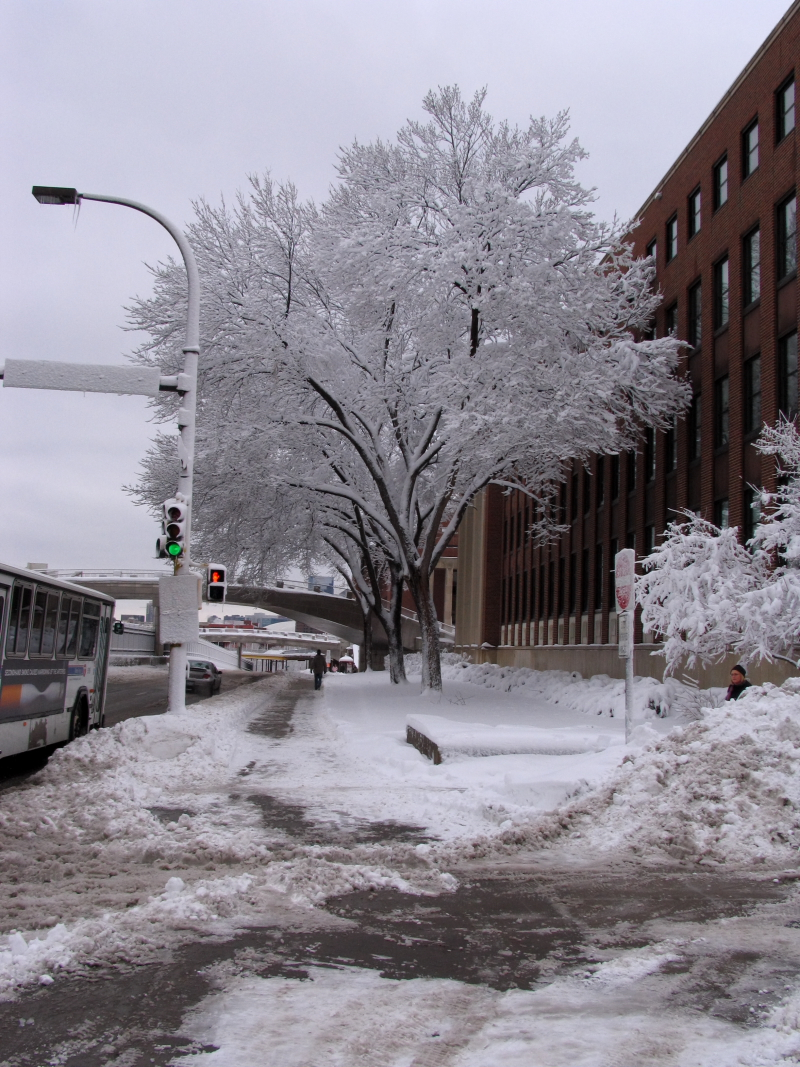
\includegraphics[width=55mm]{01/figures/mnWinter/mnWinter}\hspace{4mm}
\begin{minipage}[b]{\textwidth - 80mm}
   \caption[anecdotal evidence]{In February 2010, some media pundits cited one large snow storm as valid evidence against global warming. As comedian Jon Stewart pointed out, ``It's one storm, in one region, of one country.''\vspace{-4.5mm} \\
   
   -----------------------------\vspace{-2mm}\\
   {\footnotesize February 10th, 2010.}
   \label{mnWinter}}
\end{minipage}
\end{figure}
\setlength{\captionwidth}{\mycaptionwidth}

\begin{termBox}{\tBoxTitle{Anecdotal evidence}
Be careful of making inferences based on anecdotal evidence. Such evidence may be true and verifiable, but it may only represent extraordinary cases. The majority of cases and the average case may in fact be very different.}
\end{termBox}

\Add{
Anecdotal evidence typically is composed of unusual cases that we recall based on their striking characteristics. For instance, we may vividly remember the time when our friend bought a lottery ticket and won \$250 but forget most the times she bought one and lost.  Instead of focusing on the most unusual cases, we should examine a sample of many cases that represent the population.
}

\Comment{ subsection sampling from a population moved to section on observational studies and sampling}

\subsection{Explanatory and response variables}
\label{explanatoryAndResponse}

\index{data!county|(}

Consider the following question from page~\pageref{fedSpendingPovertyQuestion} for the \data{county} data set:
\begin{enumerate}
\item[(1)] 
	Is federal spending, on average, higher or lower in counties with high rates of poverty?
\end{enumerate}
If we suspect poverty might affect spending in a county, then poverty is the \term{explanatory} variable and federal spending is the \term{response} variable in the relationship.\footnote{Sometimes the explanatory variable is called the \term{independent} variable and the response variable is called the \term{dependent} variable. However, this becomes confusing since a \emph{pair} of variables might be independent or dependent, so we avoid this language.} If there are many variables, it may be possible to consider a number of them as explanatory variables.

\begin{tipBox}{\tipBoxTitle{Explanatory and response variables}
To identify the explanatory variable in a pair of variables, identify which of the two is suspected of affecting the other and plan an appropriate analysis.

\hspace{10mm}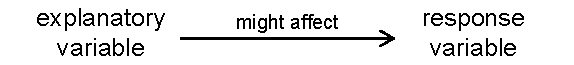
\includegraphics[height=0.34in]{01/figures/expResp/expResp}}
\end{tipBox}

\begin{caution}{association does not imply causation}{Labeling variables as \emph{explanatory} and \emph{response} does not guarantee the relationship between the two is actually causal, even if there is an association identified between the two variables. We use these labels only to keep track of which variable we suspect affects the other.}
\end{caution}

\Cut{
In some cases, there is no explanatory or response variable. Consider the following question from page~\pageref{ownershipMultiUnitQuestion}:
\begin{enumerate}
\item[(2)] 
	If homeownership is lower than the national average in one county, will the percent of multi-unit structures in that county likely be above or below the national average?
\end{enumerate}
It is difficult to decide which of these variables should be considered the explanatory and response variable, i.e. the direction is ambiguous, so no explanatory or response labels are suggested here.

\index{data!county|)}}

\Add{In some cases, the relationship is complex. It may be unclear whether variable $A$ explains variable $B$ or whether variable $B$ explains variable $A$. For example, it is now known that a particular protein called REST is much depleted in people suffering from Alzheimer's disease.  While this raises hopes of a possible approach for treating Alzheimer's, it is still unknown whether the lack of the protein causes brain deterioration, whether brain deterioration causes depletion in the REST protein, or whether some third variable causes both brain deterioration and REST depletion.  That~is, we do not know if the lack of the protein is an explanatory variable or a response variable.  Perhaps it is both.\footnote{\urlwofont{http://www.nytimes.com/2014/03/20/health/fetal-gene-may-protect-brain-from-alzheimers-study-finds.html}} }

\Comment{subsection previously titled Introducing observational studies and experiments}
\subsection{Observational studies versus experiments}

There are two primary types of data collection: observational studies and experiments.

Researchers perform an \term{observational study} when they collect data without interfering with how the data arise.  For instance, researchers may collect information via surveys, review medical or company records, or follow a \term{cohort} of many similar individuals to study why certain diseases might develop.  In each of these situations, researchers merely observe or take measurements of things that arise naturally.  

When researchers want to investigate the possibility of a causal connection, they conduct an \term{experiment}. \Add{For a study to be an experiment, the researchers must impose a treatment.} \Comment{Should this be for all experiments?} For most studies there will be both an explanatory and a response variable. For instance, we may suspect administering a drug will reduce mortality in heart attack patients over the following year. To check if there really is a causal connection between the explanatory variable and the response, researchers will collect a sample of individuals and split them into groups. The individuals in each group are \emph{assigned} a treatment. When individuals are randomly assigned to a group, the experiment is called a \term{randomized experiment}. For example, each heart attack patient in the drug trial could be randomly assigned into one of two groups: the first group receives a \term{placebo} (fake treatment) and the second group receives the drug. See the case study in Section~\ref{basicExampleOfStentsAndStrokes} for another example of an experiment, though that study did not employ a placebo.

\Comment{Can say average tip customers give or average tip a waiter receives.  My original thought was that we are interested in the behavior of the customers and that is what we are observing.}
\Add{
\begin{example}{Suppose that a researcher is interested in the average tip customers at a particular restaurant give.  Should she carry out an observational study or an experiment?} In addressing this question, we ask, ``Will the researcher be imposing any treatment?"  Because there is no treatment or interference that would be applicable here, it will be an observational study.  Additionally, one consideration the researcher should be aware of is that, if customers know their tips are being recorded, it could change their behavior, making the results of the study inaccurate.  
\end{example}
}
\begin{tipBox}{\tipBoxTitle{association $\neq$ causation}
In general, association does not imply causation, and causation can only be inferred from a randomized experiment.}
\end{tipBox}


%%%%%
\section{Observational studies and sampling strategies}

\subsection{Observational studies}

Generally, data in observational studies are collected only by monitoring what occurs, while experiments require the primary explanatory variable in a study be assigned for each subject by the researchers.

\Comment{Is it too strong to delete the word "generally" in the last sentence of this paragraph?}
Making causal conclusions based on experiments is often reasonable. However, making the same causal conclusions based on observational data is treacherous and is not recommended. Observational studies are generally only sufficient to show associations.

\Cut{
\begin{exercise} \label{sunscreenLurkingExample}
Suppose an observational study tracked sunscreen use and skin cancer, and it was found that the more sunscreen someone used, the more likely the person was to have skin cancer. Does this mean sunscreen \emph{causes} skin cancer?\footnote{No. See the paragraph following the exercise for an explanation.}
\end{exercise}
}

\Add{
\begin{exercise} \label{sunscreenLurkingExample}
Suppose an observational study tracked sunscreen use and skin cancer, and it was found people who use sunscreen are more likely to get skin cancer than people who do not use sunscreen. Does this mean sunscreen \emph{causes} skin cancer?\footnote{No. See the paragraph following the exercise for an explanation.}
\end{exercise}
}
\Comment{TODO(David) add a graphic that just shows the two boxes of sunscreen with the question mark arrow to skin cancer and a footnote that said the arrow indicates an association between sunscreen and getting skin cancer.  }

Some previous research tells us that using sunscreen actually reduces skin cancer risk, so maybe there is another variable that can explain this hypothetical association between sunscreen usage and skin cancer. One important piece of information that is absent is sun exposure. Sun exposure is what is called a \term{confounding variable}.\footnote{Also called a \term{lurking variable}, \term{confounding factor}, or a \term{confounder}.} 
\begin{center}
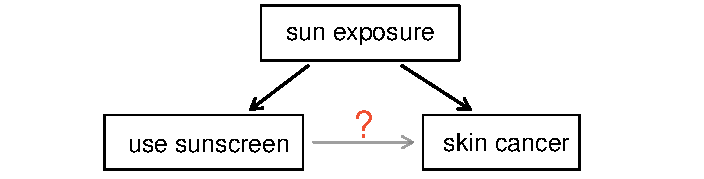
\includegraphics[height=1.0in]{01/figures/variables/sunCausesCancer}
\end{center}
% Some studies:
% http://www.sciencedirect.com/science/article/pii/S0140673698121682
% http://archderm.ama-assn.org/cgi/content/abstract/122/5/537
% Study with a similar scenario to that described here:
% http://onlinelibrary.wiley.com/doi/10.1002/ijc.22745/full



\Add{
\begin{termBox}{\tBoxTitle{\textbf{Confounding Variable}}
A confounding variable is a variable that is associated with both the explanatory \emph{and} response variables.  Because of the confounding variable's association with both variables, we do not know if the response is due to the explanatory variable or due to the confounding variable.}
\end{termBox}

Sun exposure is a confounding factor because it is associated with both the use of sunscreen and the development of skin cancer.  People who are out in the sun all day are more likely to use sunscreen \emph{and} people who are out in the sun all day are more likely to get skin cancer.  Research shows us the the development of skin cancer is due to the sun exposure.  However, without this additional research the variables of sunscreen usage and sun exposure would be \term{confounded}.  That~is without this research we would have no way of knowing which one was the true cause of skin cancer.

\begin{example}{Let's assume for the sake of argument that women are more diligent about applying sunscreen.  Would this make gender a confounding factor in this study?  } No, because there is no known association between being female and being more likely to get skin cancer.  Thus, the fact that women are more likely (in this scenario) to wear sunblock is not confounding, because it is only associated with the explanatory variable and not the response variable.  It does not explain the observed, existing association between sunblock usage and skin cancer.
\end{example}
}
\Cut{
Let's consider another example, one in which we cannot so easily tell which variable is the true cause and which is the confounding variable.  Suppose we want to test which of two colas people prefer.  We put cola A in a pink cup and cola B in a white cup.  A random sample of people take a sip of each and then report which cola they like better.  At the end of the experiment, more people preferred cola A.  Now, cola B could easily argue that people didn't really prefer the competing cola, rather they preferred the pink cup to the white cup \footnote{If this sounds silly see an almost identical, real example with Coke and Pepsi: \urlwofont{http://pirate.shu.edu/~hovancjo/exp/pepsi_coke.htm}}.  Is this true or not?  The fact is that without another experiment there is no way to say for certain whether people preferred cola A or they preferred the pink cup.  These two variables, cola type and color of cup, are \emph{confounded}.  That~is, they are impossible to untangle or to consider in isolation.  Thus we cannot know which is the cause or explanation of the response variable.   
}

While one method to justify making causal conclusions from observational studies is to exhaust the search for confounding variables, there is no guarantee that all confounding variables can be examined or measured.

In the same way, the \data{county} data set is an observational study with confounding variables, and its data cannot easily be used to make causal conclusions.

\begin{exercise}
Figure~\ref{multiunitsVsOwnership} shows a negative association between the homeownership rate and the percentage of multi-unit structures in a county. However, it is unreasonable to conclude that there is a causal relationship between the two variables. Suggest one or more other variables that might explain the relationship visible in Figure~\ref{multiunitsVsOwnership}.\footnote{Answers will vary. Population density may be important. If a county is very dense, then this may require a larger fraction of residents to live in multi-unit structures. Additionally, the high density may contribute to increases in property value, making homeownership infeasible for many residents.}
\end{exercise}

Observational studies come in two forms: prospective and retrospective studies. A \term{prospective study} identifies individuals and collects information as events unfold. For instance, medical researchers may identify and follow a group of similar individuals over many years to assess the possible influences of behavior on cancer risk. One example of such a study is The Nurses� Health Study, started in 1976 and expanded in 1989.\footnote{\urlwofont{http://www.channing.harvard.edu/nhs/}} This prospective study recruits registered nurses and then collects data from them using questionnaires. \termsub{Retrospective studies}{retrospective studies} collect data after events have taken place, e.g. researchers may review past events in medical records. Some data sets, such as \data{county}, may contain both prospectively- and retrospectively-collected variables. Local governments prospectively collect some variables as events unfolded (e.g. retails sales) while the federal government retrospectively collected others during the 2010 census (e.g. county population counts).


\subsection{Sampling from a population}

\index{sample!random sample|(}

We might try to estimate the time to graduation for Duke undergraduates in the last 5 years by collecting a sample of students. All graduates in the last 5 years represent the \emph{population}\index{population}, and graduates who are selected for review are collectively called the \emph{sample}\index{sample}. In general, we always seek to \emph{randomly} select a sample from a population. The most basic type of random selection is equivalent to how raffles are conducted. For example, in selecting graduates, we could write each graduate's name on a raffle ticket and draw 100 tickets. The selected names would represent a random sample of 100 graduates.

\begin{figure}[ht]
\centering
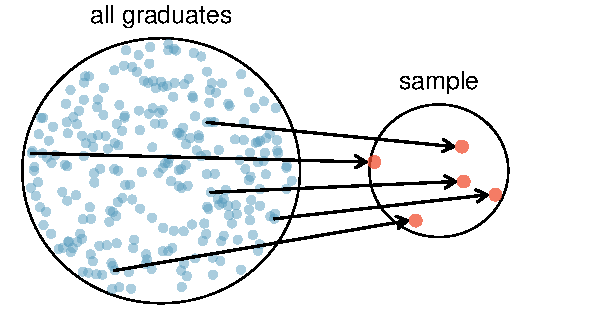
\includegraphics[width=0.47\textwidth]{01/figures/popToSample/popToSampleGraduates}
\caption{In this graphic, five graduates are randomly selected from the population to be included in the sample.}
\label{popToSampleGraduates}
\end{figure}

Why pick a sample randomly? Why not just pick a sample by hand? Consider the following scenario.

\begin{example}{Suppose we ask a student who happens to be majoring in nutrition to select several graduates for the study. What kind of students do you think she might collect? Do you think her sample would be representative of all graduates?}
Perhaps she would pick a disproportionate number of graduates from health-related fields. Or perhaps her selection would be well-representative of the population. When selecting samples by hand, we run the risk of picking a \emph{biased} sample, even if that bias is unintentional or difficult to discern.
\end{example}

\begin{figure}
\centering
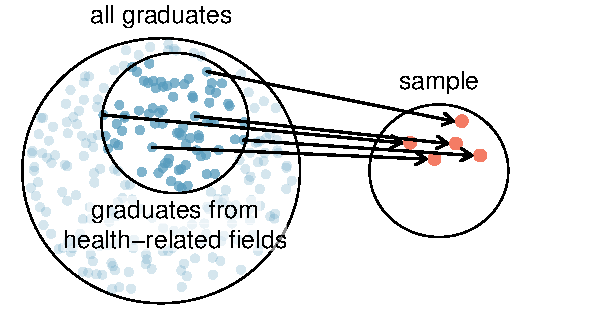
\includegraphics[width=0.47\textwidth]{01/figures/popToSample/popToSubSampleGraduates}
\caption{Instead of sampling from all graduates equally, a nutrition major might inadvertently pick graduates with health-related majors disproportionately often.}
\label{popToSubSampleGraduates}
\end{figure}

\Comment{example reworded to emphasize what specific effect the bias would have on the estimate}
\Add{
If the student majoring in nutrition picked a disproportionate number of graduates from health-related fields, this would introduce \term{selection bias} into the sample. Selection bias occurs when some individuals of the population are more likely to be included in the sample than others.  This is a problem because a degree in health-related fields might take more or less time to complete than a degree in other fields.  Suppose that it takes longer.  Since graduates from health-related fields would be more likely to be in the sample, the selection bias would cause her to \emph{overestimate} the parameter.} Sampling randomly helps resolve this problem. The most basic random sample is called a \term{simple random sample}, and it is the equivalent of using a raffle to select cases. This means that each case in the population has an equal chance of being included and there is no implied connection between the cases in the sample.  \Add{If a simple random sample is chosen from the entire population of interest, there is no human or selection bias introduced.}

\Cut{
\APVersion{Sometimes a simple random sample is difficult to implement and an alternative method is helpful. One such substitute is a \term{systematic sample}, where one case is sampled after letting a fixed number of others, say 10 other cases, pass by. Since this approach uses a mechanism that is not easily subject to personal biases, it often yields a reasonably representative sample. This book will focus on random samples since the use of systematic samples is uncommon and requires additional considerations of the context.}{}
}

\begin{figure}[h]
\centering
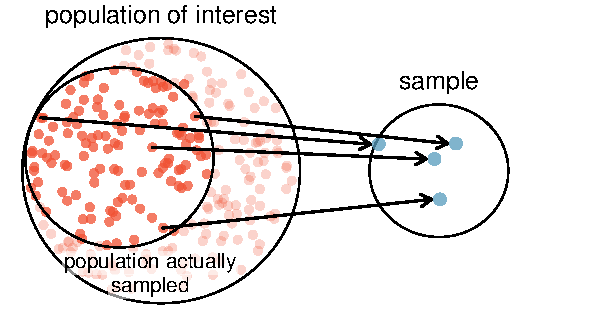
\includegraphics[width=0.5\textwidth]{01/figures/popToSample/surveySample}
\caption{Due to the possibility of non-response, surveys studies may only reach a certain group within the population. It is difficult, and often times impossible, to completely fix this problem.}
\label{surveySample}
\end{figure}

A common downfall is a \term{convenience sample}\index{sample!convenience sample}, where individuals who are easily accessible are more likely to be included in the sample. For instance, if a political survey is done by stopping people walking in the Bronx, this will not represent all of New York City. It is often difficult to discern what sub-population a convenience sample represents. 

\Add{
Similarly, a \term{volunteer sample} is one in which people's responses are solicited and those who choose to participate, respond.  This is a problem because those who choose to participate may tend to have different opinions than the rest of the population, resulting in a biased sample.  
}

\begin{exercise}
We can easily access ratings for products, sellers, and companies through websites. These ratings are based only on those people who go out of their way to provide a rating. If 50\% of online reviews for a product are negative, do you think this means that 50\% of buyers are dissatisfied with the product?\footnote{Answers will vary. From our own anecdotal experiences, we believe people tend to rant more about products that fell below expectations than rave about those that perform as expected. For this reason, we suspect there is a negative bias in product ratings on sites like Amazon. However, since our experiences may not be representative, we also keep an open mind should data on the subject become available.}
\end{exercise}

The act of taking a random sample helps minimize bias; however, bias can crop up in other ways.  Even when people are picked at random, e.g. for surveys, caution must be exercised if the \term{non-response} \index{sample!non-response|textbf} is high.  For instance, if only 30\% of the people randomly sampled for a survey actually respond, then it is unclear whether the results are \term{representative} of the entire population. This \term{non-response bias} \index{sample!non-response bias|textbf} can skew results.

\Add{
Even if a sample has no selection bias and no non-response bias, there is an additional type of bias that often crops up and undermines the validity of results, known as response bias.  \termsub{Response bias}{response bias} refers to a broad range of factors that influence how a person responds, such as wording of the question, order of the questions, and influence of the interviewer.  This type of bias can be present even when we collect data from an entire population in what is called a \term{census}.  Because response bias is often subtle, one must pay careful attention to how questions were asked when attempting to draw conclusions from the data.

\begin{example}{Suppose a high school student wants to investigate the student body's opinions on the food in the cafeteria.  Let's assume that she manages to survey every student in the school.  How might response bias arise in this context?}There are many possible correct answers to this question.  For example, students might respond differently depending upon who asks the question, such as a school friend or someone who works in the cafeteria.  The wording of the question could introduce response bias.  Students would likely respond differently if asked ``Do you like the food in the cafeteria?" versus ``The food in the cafeteria is pretty bad, don't you think?".  
\end{example}


\begin{tipBox}{\tipBoxTitle{Watch out for bias}
Selection bias, non-response bias, and response bias can still exist within a random sample.  Always ask how a sample was chosen, whether anyone failed to respond (and if so, how many people failed to respond), and critically examine the wording of the questions.}
\end{tipBox}

When there is no bias in a sample, increasing the sample size tends to increase the precision and reliability of the estimate.  When a sample is biased, it may be impossible to decipher helpful information from the data, even if the sample is very large.  

}
\Comment{This can be omitted if it seems too obvious.  I was trying to emphasize the fact that increasing the sample size does not fix the problem of bias}
\Add{
\begin{exercise}A researcher sends out questionnaires to 50 randomly selected households in a particular town asking whether or not they support the addition of a traffic light in their neighborhood.  Because only 20\% of the questionaires are returned, she decides to mail questionnaires to 50 more randomly selected households in the same neighborhood.  Comment on the usefulness of this approach.\footnote{Sampling more people does nothing to eliminate the non-response bias because the same type of people who did not respond to the first sample are likely to not respond in the new sample. Instead, she should make an effort to reach out to the households from the original sample that did not respond and solicit their feedback, possibly by going door to door.}
\end{exercise}
}



\index{sample!random sample|)}
\index{population|)}
\index{sample|)}


\subsection{Simple, systematic, stratified, cluster, and multistage sampling}
\label{threeSamplingMethods}

\Cut{
Almost all statistical methods are based on the notion of implied randomness. If observational data are not collected in a random framework from a population, these statistical methods -- the estimates and errors associated with the estimates -- are not reliable. Here we consider three random sampling techniques: simple, stratified, and cluster sampling. Figure~\ref{simple_systematic} provides a graphical representation of these techniques.}

\Add{
Almost all statistical methods for observational data rely on a sample being random and unbiased. When a sample is collected in a biased way, these statistical methods will generally not produce reliable information about the population

The idea of a simple random sample was introduced in the last section.  Here we provide a more technical treatment of this method and introduce four new random sampling methods:  systematic, stratified, cluster, and multistage.\footnote{Systematic and Multistage sampling are not part of the AP syllabus.} Figure~\ref{simple_systematic} provides a graphical representation of simple versus systematic sampling while Figure~\ref{stratified_cluster_multistage} provides a graphical representation of stratified, cluster, and multistage sampling.
}

\begin{figure}
\centering
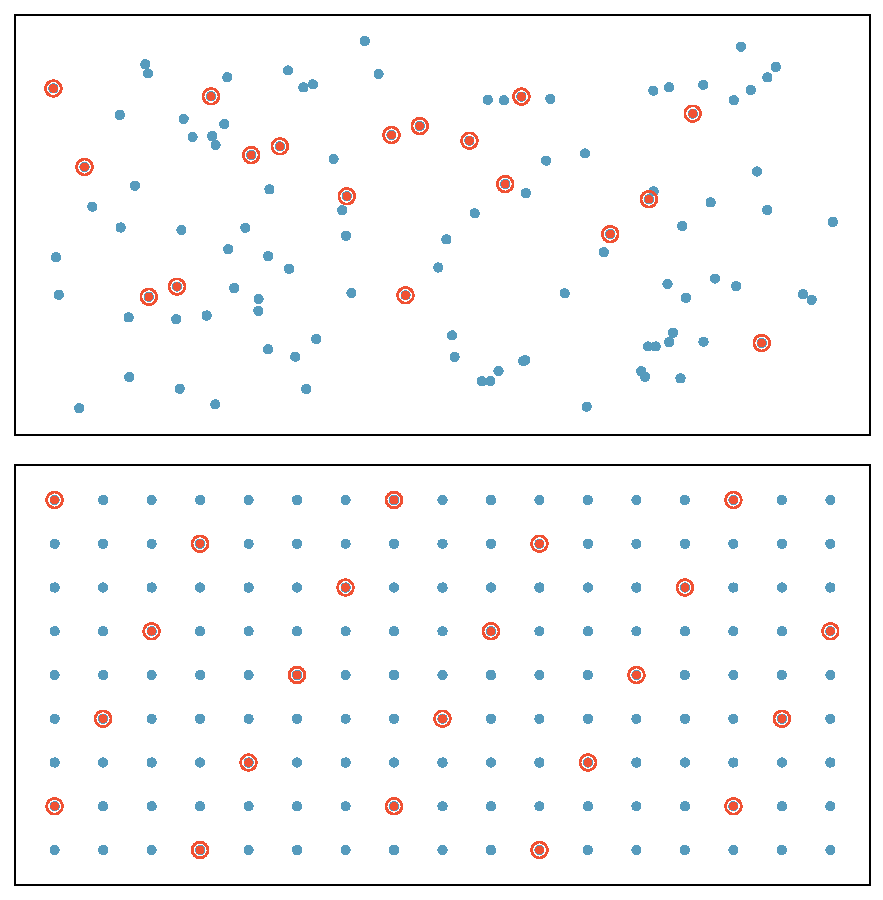
\includegraphics[width=0.8\textwidth]{01/figures/samplingMethodsFigure/simple_systematic}
\caption{Simple versus stratified random sampling.  In the top panel, simple random sampling was used to randomly select 18 cases.  In the lower panel, systematic random sampling was used to select every 7th individual.}
\label{simple_systematic}
\end{figure}

\termsub{Simple random sampling}{sample!simple random sampling} is probably the most intuitive form of random sampling. Consider the salaries of Major League Baseball (MLB) players, where each player is a member of one of the league's 30 teams. \Cut{To take a simple random sample of 120 baseball players and their salaries from the 2010 season, we could write the names of that season's 828 players onto slips of paper, drop the slips into a bucket, shake the bucket around until we are sure the names are all mixed up, then draw out slips until we have the sample of 120 players. In general, a sample is referred to as ``simple random'' if each case in the population has an equal chance of being included in the final sample \emph{and} knowing that a case is included in a sample does not provide useful information about which other cases are included.}  \Add{For the 2010 season, N, the population size or total number of players, is 828.  To take a simple random sample of \textit{n} = 120 of these baseball players and their salaries, we could number each player from 1 to 828.  Then we could randomly select 120 numbers between 1 and 828 (without replacement) using a random number generator or random digit table.  The players with the selected numbers would comprise our sample.  

\par In a ``simple random sample" two properties are always true.  
\begin{itemize} 
\item Property 1:  Each case in the population has an equal chance of being included in the final sample
\item Property 2:  Each \emph{group} of \textit{n} cases has an equal chance of making up the sample.  
\end{itemize}

The statistical methods in this book focus on data collected using simple random sampling.  Note that Property 2: Each group of \textit{n} cases has an equal chance making up the sample is not true for the remaining four sampling techniques.  As you read each one, consider why.
}
\Comment{I have reworded a little bit of this try to make for better paragraph transitions, and added some exercises to break up the monotony of the paragraphs.  Also, I standardized the bold faced terms so they all use "sampling" rather than some use sample and some use sampling.}

\Add{
Though less common than simple random sampling, \termsub{systematic sampling}{sample!systematic sampling} is sometimes used when there exists a convenient list of all of the individuals of the population.   Suppose we have a roster with the names of all the MLB players from the 2010 season.  To take a systematic random sample, number them from 1 to 828.  Select one random number between 1 and 828 inclusive and let that player be the first individual in the sample.  Then, depending on the desired sample size, select every 10th number or 20th number, for example, to arrive at the sample.\footnote{If we want a sample of size \textit{n} = 138, it would make sense to select every 6th player since 828/138 = 6.  Suppose we randomly select the number 810.  Then player 810, 816, 822, 828, 6, 12, $\cdots$ , 798, and 804 would make up the sample.} If there are no patterns in the salaries based on the numbering then this could be a reasonable method.  

\begin{exercise}
A systematic sample is not the same as a simple random sample. Provide an example of a sample that can come from a simple random sample but not from a systematic random sample.\footnote{Answers will vary. If we take a sample of size 3, then it is possible that we could sample players numbered 1, 2, and 3 in a simple random sample. Such a sample would be impossible from a systematic sample.  Property 2 of simple random samples does not hold for other types of random samples.}
\end{exercise}

\begin{figure}
\centering
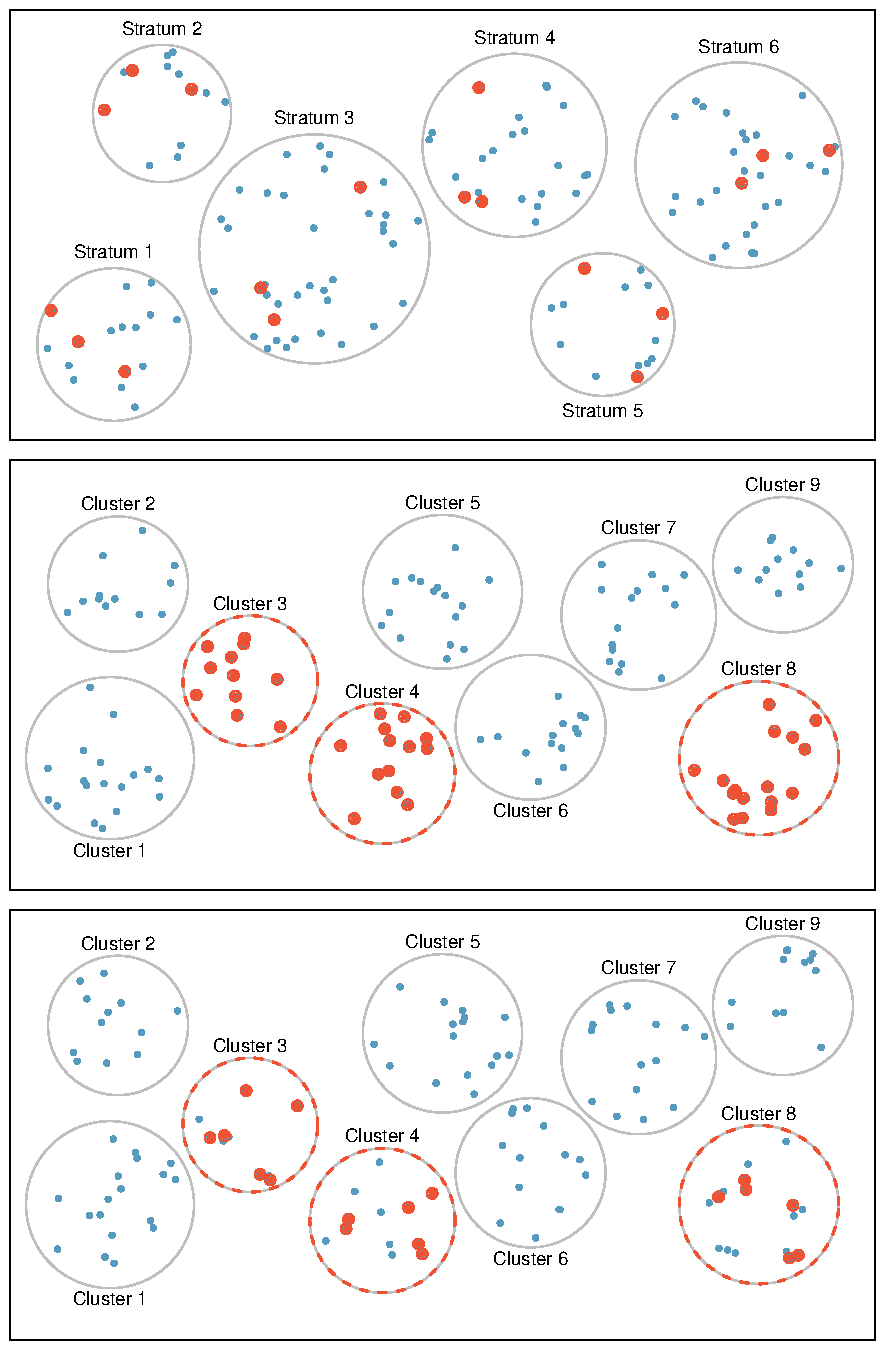
\includegraphics[width=0.8\textwidth]{01/figures/samplingMethodsFigure/stratified_cluster_multistage}
\caption{Examples of stratified, cluster, and multistage sampling. In the top panel, stratified sampling was used: cases were grouped into strata, and then simple random sampling was employed within each stratum.  In the middle panel, cluster sampling was used, where data were binned into nine cluster and three clusters were randomly selected.  In the bottom panel, multistage cluster sampling was used.  Data were binned into the nine clusters, three of the cluster were randomly selected, and then six cases were randomly sampled in each of the three selected clusters.}
\label{stratified_cluster_multistage}
\end{figure}

Sometimes there is a variable that is known to be associated with the quantity we want to estimate.  In this case, a stratified random sample might be selected.  \termsub{Stratified sampling}{sample!stratified sampling} is a divide-and-conquer sampling strategy. The population is divided into groups called \term{strata}\index{sample!strata|textbf}. The strata are chosen so that similar cases are grouped together and a sampling method, usually simple random sampling, is employed to select a certain number or a certain proportion of the whole within each stratum. In the baseball salary example, the 30 teams could represent the strata; some teams have a lot more money (we're looking at you, Yankees).  

\begin{example}{For this baseball example, briefly explain how to select a stratified random sample of size \textit{n} = 120. }
Because each team is a stratum, we could take a simple random sample of 4 players from each of the 30 teams, yielding a sample of 120 players.
\end{example}

Stratified sampling is inherently different than simple random sampling. For example, the stratified sampling approach described would make it impossible for the entire Yankees team to be included in the sample.
}

\Cut{
Stratified sampling is especially useful when the cases in each stratum are very similar \emph{with respect to the outcome of interest}. In a simple random sample, it is possible that just by random chance we could end up with proportionally too many Yankees players in our sample, thus overestimating the true average salary of all MLB players. A stratified random sample would assure proportional representation from each team.

The downside is that analyzing data from a stratified sample is a more complex task than analyzing data from a simple random sample. The analysis methods introduced in this book would need to be extended to analyze data collected using stratified sampling.

\begin{example}{Why is it good for cases within each stratum to be very similar?}
We should get a more stable estimate for the subpopulation in a stratum if the cases are very similar. These improved estimates for each subpopulation will help us build a reliable estimate for the full population.
\end{example}
}

\Add{
\begin{example}{Stratified sampling is especially useful when the cases in each stratum are very similar \emph{with respect to the outcome of interest}.  Why is it good for cases within each stratum to be very similar?}
We should get a more stable estimate for the subpopulation in a stratum if the cases are very similar. These improved estimates for each subpopulation will help us build a reliable estimate for the full population.  For example, in a simple random sample, it is possible that just by random chance we could end up with proportionally too many Yankees players in our sample, thus overestimating the true average salary of all MLB players. A stratified random sample can assure proportional representation from each team.
\end{example}
}


\Cut{
A \termsub{cluster sample}{sample!cluster sample} is much like a two-stage simple random sample. We break up the population into many groups, called \termsub{clusters}{sample!cluster}. Then we sample a fixed number of clusters and collect a simple random sample within each cluster. This technique is similar to stratified sampling in its process, except that there is no requirement in cluster sampling to sample from every cluster. Stratified sampling requires observations be sampled from every stratum.

Sometimes cluster sampling can be a more economical random sampling technique than the alternatives. Also, unlike stratified sampling, cluster sampling is most helpful when there is a lot of case-to-case variability within a cluster but the clusters themselves don't look very different from one another. For example, if neighborhoods represented clusters, then this sampling method works best when the neighborhoods are very diverse. A downside of cluster sampling is that more advanced analysis techniques are typically required, though the methods in this book can be extended to handle such data.}

\Add{
Next, let's consider a sampling technique that randomly selects groups of people.  \termsub{Cluster sampling}{sample!cluster sampling} is much like simple random sampling, but instead of randomly selecting \emph{individuals}, we randomly select groups or \term{clusters}.  Unlike stratified sampling, cluster sampling is most helpful when there is a lot of case-to-case variability within a cluster but the clusters themselves don't look very different from one another.  That~is, we expect strata to be self-similar (homogeneous), while we expect clusters to be diverse (heterogeneous). 

Sometimes cluster sampling can be a more economical random sampling technique than the alternatives.  For example, if neighborhoods represented clusters, this sampling method works best when each neighborhood is very diverse. Because each neighborhood itself encompasses diversity, a cluster sample can reduce the time and cost associated with data collection, because the interviewer would need only go to some of the neighborhoods rather than to all parts of a city, in order to get a representative sample.

\termsub{Multistage sampling}{sample!multistage sampling},  or \termsub{multistage cluster sampling}{sample!multistage cluster sampling} is a two (or more) step strategy. The first step is to take a cluster sample, as described above.  Then, instead of including all of the individuals in these clusters in our sample, a second sampling method, usually simple random sampling, is employed within each of the \emph{selected} clusters.  In the neighborhood example, we could first randomly select some number of neighborhoods and then take a simple random sample from just those selected neighborhoods.  As can be seen in Figure~\ref{samplingMethodsFigure}, stratified sampling requires observations be sampled from \emph{every} stratum.  Multistage sampling selects observations \emph{only} from those clusters that were randomly selected in step 1.  

It is also possible to have more than two steps in multistage sampling.  Each cluster may be naturally divided into subclusters.  For example, each neighborhood could be divided into streets.  To take a three-stage sample, we could first select some number of clusters (neighborhoods), and then, within the selected clusters, select some number of subclusters (streets).  Finally, we could select some number of individuals from each of the selected streets.  

}

\begin{example}{Suppose we are interested in estimating the malaria rate in a densely tropical portion of rural Indonesia. We learn that there are 30 villages in that part of the Indonesian jungle, each more or less similar to the next. Our goal is to test 150 individuals for malaria. What sampling method should be employed?}
A simple random sample would likely draw individuals from all 30 villages, which could make data collection extremely expensive. Stratified sampling would be a challenge since it is unclear how we would build strata of similar individuals. However, multistage cluster sampling seems like a very good idea. First, we might randomly select half the villages, then randomly select 10 people from each. This would probably reduce our data collection costs substantially in comparison to a simple random sample and would still give us reliable information.
\end{example}

\begin{caution}{advanced sampling techniques require advanced methods}{The methods of inference covered in this book generally only apply to simple random samples. More advanced analysis techniques are required for systematic, stratified, cluster, and multistage random sampling.}
\end{caution}


%%%%%
\section{Experiments}
\label{experimentsSection}
\Cut{
Studies where the researchers assign treatments to cases are called \termsub{experiments}{experiment}. When this assignment includes randomization, e.g. using a coin flip to decide which treatment a patient receives, it is called a \term{randomized experiment}. Randomized experiments are fundamentally important when trying to show a causal connection between two variables.
}

\Add{
In the last section we investigated observational studies and sampling strategies.  While these are effective tools for answering certain research questions, often times researchers want to measure the effect of a treatment.  In this case, they must carry out an experiment.  Just as randomization is essential in sampling in order to avoid selection bias, randomization is essential in the context of experiments to determine which subjects will receive which treatments.  If the researcher chooses who gets a new treatment, she may unintentionally select healthier or sicker patients to get the treatment, biasing the experiment either for or against the treatment.  
}
\Comment{The wording of previous sentence is a bit awkward, but I want to try to always force reader to think about the direction of the bias, not just that there will be bias, as ap questions always require students to explain how (meaning in which direction) it will bias estimate.} 

\Comment{principles of experimental design subsection moved to follow reducing bias section}

\subsection{Reducing bias in human experiments}
\label{biasInHumanExperiments}

\Cut{Randomized experiments are the gold standard for data collection, but they do not ensure an unbiased perspective into the cause and effect relationships in all cases. }
\Add{Randomized experiments are essential for investigating cause and effect relationships, but they do not ensure an unbiased perspective in all cases.}  Human studies are perfect examples where bias can unintentionally arise. Here we reconsider a study where a new drug was used to treat heart attack patients.\footnote{Anturane Reinfarction Trial Research Group. 1980. Sulfinpyrazone in the prevention of sudden death after myocardial infarction. New England Journal of Medicine 302(5):250-256.} In particular, researchers wanted to know if the drug reduced deaths in patients.

These researchers designed a randomized experiment because they wanted to draw causal conclusions about the drug's effect. Study volunteers\footnote{Human subjects are often called \term{patients}, \term{volunteers}, or \term{study participants}.} were randomly placed into two study groups. One group, the \term{treatment group}, received the drug. The other group, called the \term{control group}, did not receive any drug treatment. \Add{  In an experiment, the explanatory variable is also called a \term{factor}.  Here the factor is receiving the drug treatment.  It has two \term{levels}:  yes and no, thus it is categorical.  The response variable is whether or not patients died within the time frame of the study.  It is also categorical.}

Put yourself in the place of a person in the study. If you are in the treatment group, you are given a fancy new drug that you anticipate will help you. On the other hand, a person in the other group doesn't receive the drug and sits idly, hoping her participation doesn't increase her risk of death. These perspectives suggest there are actually two effects: the one of interest is the effectiveness of the drug, and the second is an emotional effect that is difficult to quantify.

Researchers aren't usually interested in the emotional effect, which might bias the study. To circumvent this problem, researchers do not want patients to know which group they are in. When researchers keep the patients uninformed about their treatment, the study is said to be \term{blind} or \term{single-blind}. But there is one problem: if a patient doesn't receive a treatment, she will know she is in the control group. The solution to this problem is to give fake treatments to patients in the control group. A fake treatment is called a \term{placebo}, and an effective placebo is the key to making a study truly blind. A classic example of a placebo is a sugar pill that is made to look like the actual treatment pill. Often times, a placebo results in a slight but real improvement in patients. This effect has been dubbed the \term{placebo~effect}.

The patients are not the only ones who should be blinded: doctors and researchers can accidentally bias a study. When a doctor knows a patient has been given the real treatment, she might inadvertently give that patient more attention or care than a patient that she knows is on the placebo. To guard against this bias, which again has been found to have a measurable effect in some instances, most modern studies employ a \term{double-blind} setup where researchers who interact with subjects and are responsible for measuring the response variable are, just like the subjects, unaware of who is or is not receiving the treatment.\footnote{There are always some researchers involved in the study who do know which patients are receiving which treatment. However, they do not interact with the study's patients and do not tell the blinded health care professionals who is receiving which treatment.} 


\begin{exercise}
Look back to the study in Section~\ref{basicExampleOfStentsAndStrokes} where researchers were testing whether stents were effective at reducing strokes in at-risk patients. Is this an experiment? Was the study blinded? Was it double-blinded?\footnote{The researchers assigned the patients into their treatment groups, so this study was an experiment. However, the patients could distinguish what treatment they received, so this study was not blind. The study could not be double-blind since it was not blind.}
\end{exercise}

\Comment{this section can be omitted as it might be interesting, but not relevant}

\Add{Randomized, controlled, double-blind experiments are the gold standard of data collection, so much so that this method is being employed to investigate the efficacy of certain surgical procedures. Placebo surgery, also known as ``sham"' surgery, is a controversial but existing practice wherein subjects undergo a real surgical intervention but do not receive the treatment or therapy being investigated.  
\begin{example}{Placebo surgery has been used in evaluating surgical procedures for, most notably, Parkinson Disease, knee injury, and back pain.  Describe some arguments for and against using a placebo surgery.}In these situations, the response variable being measured is not an objective yes or no.  It is a continuum of pain or debilitation.  Without a placebo, the researchers cannot be entirely confident that any improvement from the surgery is not partially or entirely due to the placebo effect.  Because the surgery is costly and can involve complications, doctors (and insurance companies) want to be certain that it is truly effective before carry it out on a large number of patients.  However, all surgeries involve some inherent risk.  There is debate in the medical community as to whether the knowledge that can be gained from these placebo surgeries justifies the risk posed to the patients.\footnote{Read more about this topic here: \urlwofont{http://www.ncbi.nlm.nih.gov/pmc/articles/PMC3703438/}
}
\end{example}

}  

\subsection{Principles of experimental design}
\label{experimentalDesignPrinciples}

\Add{Well-conducted experiments are built on three main principles.}
\Cut{Randomized experiments are generally built on four principles.} 

\begin{description}
\item[\term{Direct Control}] Researchers assign treatments to cases, and they do their best to \term{control} any other differences in the groups. \Add{They want the groups to be as identical as possible \emph{except for the treatment}, so that at the end of the experiment any difference in response between the groups can be attributed to the treatment and not to some other confounding or luking variable}. For example, when patients take a drug in pill form, some patients take the pill with only a sip of water while others may have it with an entire glass of water. To control for the effect of water consumption, a doctor may ask all patients to drink a 12 ounce glass of water with the pill. \Add{Direct control refers to variables that the researcher can control, or make the same.  A researcher can directly control the appearance of the treatment, the time of day it is taken, etc.  She cannot directly control variables such as gender or age.  To control for variables such as these, she might consider blocking, as described in the section that follows.}
\item[Randomization.] Researchers randomize patients into treatment groups to account for variables that cannot be controlled. For example, some patients may be more susceptible to a disease than others due to their dietary habits. Randomizing patients into the treatment or control group helps \emph{even out}  the effects of such differences, and it also prevents accidental bias from entering the study.  
\item[Replication.] The more cases researchers observe, the more accurately they can estimate the effect of the explanatory variable on the response. \Add{In an experiment with six subjects, even if there is randomization, it is quite possible for the three healthiest people to be in the same treatment group. In a randomized experiment with 100 people, it is practically impossible for the healthiest 50 people to end up in the same treatment group.  In a single study, we \term{replicate} by imposing the treatment on a sufficiently large number of subjects or experimental units. A group of scientists may replicate an entire study to verify an earlier finding, but each study should ensure a sufficiently large number of subjects because, in many cases, there is no opportunity or funding to carry out the entire experiment again.}  \Cut{In a single study, we \term{replicate} by collecting a sufficiently large sample. Additionally, a group of scientists may replicate an entire study to verify an earlier finding.}
\end{description}

\Add{It is important to incorporate these design principles into any experiment.  If they are lacking, the inference methods presented in the following chapters will not be applicable and their results will not be trustworthy.  In the next section we will consider three types of experimental design.}

\Cut{
It is important to incorporate the first three experimental design principles into any study, and this book describes applicable methods for analyzing data from such experiments. Blocking is a slightly more advanced technique, and statistical methods in this book may be extended to analyze data collected using blocking.
}
\Comment{blocking moved to next section}

\subsection{Completely randomized, blocked, and matched pairs design}
\index{completely!randomized|)}
\index{blocked!experiment)}
\index{matched!pairs|)}

\Add{
A \term{completely randomized experiment} is one in which the subjects or experimental units are randomly assigned to each treatment group.  One of the treatment groups may be given a  placebo.  Suppose we have three treatments and 300 subjects.  To carry out a completely randomized design, we could \emph{randomly} assign each subject a unique number from 1-300, then subjects with numbers 1-100 would get treatment 1, subjects 101-200 would get treatment 2, and subjects 201- 300 would get treatment 3.  Note that this method of randomly allocating subjects to treatments in not equivalent to taking a simple random sample.  Here we are not sampling a subset of a population; we are randomly \emph{splitting} subjects into groups.   

\Comment{TODO(David)a graphic here would be nice - see APprobBlocking.pdf that I put on AP Statistics dropbox for example of diagram (doesn't need to be exactly like that.}


\Comment{for ap exam, even though it seems obvious, students need to explicitly explain the method of assigning treatments to groups using specific numbers.  they also are not allowed to say -have each roll a die and...because they could end up with unequal group sizes unless they specifically explain how to avoid that (again, obvious)}

While it might be ideal for the subjects to be a random sample of the entire population of interest, that is almost never the case.  Subjects must volunteer to be part of an experiment.  However, because randomization is incorporated in the splitting of the groups, the inference procedures of this book can still be used.  Keep in mind, though, that the population to which the inference can be made might be limited.  For example, if an experiment only involves young people, the results may not be applicable to older people.   }

\begin{figure}
\centering
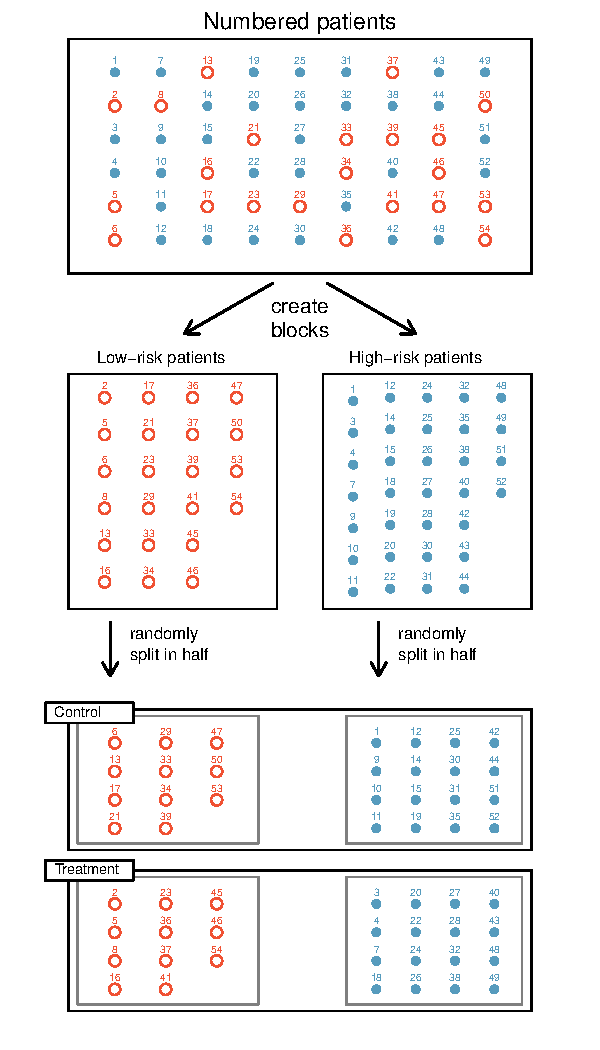
\includegraphics[width=0.78\textwidth]{01/figures/figureShowingBlocking/figureShowingBlocking}
\caption{Blocking using a variable depicting patient risk. Patients are first divided into low-risk and high-risk blocks, then each block is evenly separated into the treatment groups using randomization. This strategy ensures an equal representation of patients in each treatment group from both the low-risk and high-risk categories.}
\label{figureShowingBlocking}
\end{figure}

\Comment{TODO( David), could you redo blocking figure and have the whole group without numbers, then have each block numbered separately, in random order, then have the first however many numbers be in treatment and the remaining in control?   Also, can you two arrows coming out of each block pointing to control and treatment?  See APprobBlocking.pdf on AP Statistics dropbox for an example of what I mean.}

\Cut{Researchers sometimes know or suspect that variables, other than the treatment, influence the response. Under these circumstances, they may first group individuals based on this variable into \term{blocks} and then randomize cases within each block to the treatment groups. This strategy is often referred to as \term{blocking}. For instance, if we are looking at the effect of a drug on heart attacks, we might first split patients in the study into low-risk and high-risk blocks, then randomly assign half the patients from each block to the control group and the other half to the treatment group, as shown in Figure~\ref{figureShowingBlocking}. This strategy ensures each treatment group has an equal number of low-risk and high-risk patients.}

\Add{Researchers sometimes know or suspect that another variable, other than the treatment, influences the response. Under these circumstances, they may carry out a \term{blocked experiment}.  In this design, they first group individuals into \term{blocks} based on the identified variable and then randomize subjects within each block to the treatment groups. This strategy is referred to as \term{blocking}. For instance, if we are looking at the effect of a drug on heart attacks, we might first split patients in the study into low-risk and high-risk blocks, then randomly assign half the patients from each block to the control group and the other half to the treatment group, as shown in Figure~\ref{figureShowingBlocking}.  At the end of the experiment we compare \emph{within} blocks, that~is, we will compare low-risk patients to low-risk patients and high-risk patients to high-risk patients.  By blocking by risk of patient, we control for this possible confounding factor.  Additionally, by randomizing subjects to treatments within each block, we attempt to even out the effect of variables that we cannot block or directly control.

\begin{example}{An experiment will be conducted to compare the effectiveness of two methods for quitting smoking.  Identify a variable that the researcher might wish to use for blocking and describe how she would carry out a blocked experiment.}{The researcher should choose the variable that is most likely to influence the response variable - whether or not a smoker will quit. A reasonable variable, therefore, would be the number of years that the smoker has been smoking.  The subjects could be separated into three blocks based on number of years of smoking.  Within each block, half of the subjects would be randomly selected to receive the first treatment and the other half would receive the second treatment. }
\end{example} 

Even in a blocked experiment with randomization, other variables that affect the response can be distributed unevenly among the treatment groups, thus biasing the experiment in one direction.  A third type of design, known as \term{matched pairs} addresses this problem.  In a matched pairs experiment, pairs of people are matched on as many variables as possible, so that the comparison happens between very similar cases.  This is actually a special type of blocked experiment, where the blocks are of size two. 

\Comment{TODO(David), maybe add a graphic here for matched pairs that shows two columns of numbers with a footnote that says the subjects are compared pairwise, rather than first aggregrating the results of each group and then comparing.}

An alternate form of matched pairs involves each subject receiving \emph{both} treatments. Randomization can be incorporated by randomly selecting half the subjects to receive treatment 1 first, followed by treatment 2, while the other half receives treatment 2 first, followed by treatment 1.  Why is randomization important in this context?\footnote{Assume that all subjects received treatment 1 first, followed by treatment 2.  If the variable being measured happens to increase naturally over the course of time, it would appear as though treatment 2 had a greater effect than it really did.}

This type of matched pairs design is optimal, because it allows us to compare each subject to herself, rather than comparing a group of subjects to a separate group of subjects.  By doing this, we control for the inherent variability in response from person to person.  

\begin{exercise}
Matched pairs sometimes involves each subject receiving both treatments at the same time.  For example, if a hand lotion was being tested, half of the subjects could be randomly assigned to put Lotion A on the left hand and Lotion B on the right hand, while the other half of the subjects would put Lotion B on the left hand and Lotion A on the right hand.  Why would this be a better design than a completely randomized experiment in which half of the subjects put Lotion A on both hands and the other half put Lotion B on both hands?\footnote{The dryness of people's skins varies significantly from person to person, but less so from one person's right hand to left hand.  Thus, with the matched pairs design you are able to control for the variability in skin dryness from person to person by comparing each person's skin her own skin.  In a completely randomized experiment, it is possible that one group, just by chance, could have more people with especially dry skin, thus biasing the results against the lotion that they used.}
\end{exercise}

Because it is essential to identify the type of data collection method used when choosing an appropriate inference procedure, we will revisit sampling techniques and experiment design in the subsequent chapters on inference.  
}

\Add{
\subsection{Testing more than one variable at a time}

\Comment{a don't think factorial experiment needs to be a term since they do not need no that term, just be able to identify how many factors a experiment has.  can rewrite to say, "Instead, we want to do an experiment in which"}

Some experiments study more than one factor (explanatory variable) at a time, and each of these factors may have two or more levels (possible values).  For example, suppose a researcher plans to investigate how type and volume of music affect one's performance on a particular video game. Because these two factors, type and volume, could interact in interesting ways, we do not want to do two separate experiments testing one factor at time.  Instead, we want to do a factorial experiment in which we test all the \emph{combinations} of the factors.  Let's say that volume has two levels: soft and loud and that type has three levels:  dance, classical, and punk. Then, we would want to carry out the experiment at each of the six (2 x 3 = 6) combinations:  soft dance, soft classical, soft punk, loud dance, loud classical, loud punk.  Each of the these combinations is a \term{treatment}.  Therefore, this experiment will have 2 factors and 6 treatments.  In order to replicate each treatment 10 times, one would need to play the game 60 times.

\begin{exercise}A researcher wants to compare the effectiveness of four different drugs.  She also wants to test each of the drugs at two doses: low and high.  Describe the factors, levels, and treatments of this experiment.\footnote{There are two factors: type of drug, which has four levels, and dose, which has 2 levels.  There will be 4 x 2 = 8 treatments (drug 1 at low dose, drug 1 at high dose, drug 2 at low dose, etc.)}
\end{exercise}

As the number of factors and levels increases, the number of treatments become large and the analysis of the resulting data becomes more complex, requiring the use of advanced statistical methods.  We will investigate only one factor at a time in this book.
}

\Comment{examining data moved to its own chapter, 01b for now.  I simply copied everything into the new folder 01b and deleted the repetiitons of text and exercises}
